Using logic grid puzzles as a use-case, we validate the feasibility of finding a non-redundant explanation sequence.
As data we use puzzles from Puzzle Baron’s Logic Puzzles Volume 3~\cite{logigrammen}. The first 10 puzzles were used to construct the grammar; the next 10 to test the genericity of the grammar. 
Our experiments below are on test puzzles only; we also report results on the \textit{pasta} puzzle, which was sent to us by someone who did not manage to solve it himself.

As constraint solving engine, we use \idp~\cite{IDP} for the reasons explained in Section \ref{sec:holistic}. 
The algorithm itself is written in embedded LUA, which provides an imperative environment inside the otherwise declarative \idp system. The code was not optimized for efficiency and can at this point not be used in an interactive setting, as it takes between 15 minutes to a few hours to fully explain a logic grid puzzle. Experiments were run on an Intel(R) Xeon(R) CPU E3-1225 with 4 cores and 32 Gb memory, running linux 4.15.0 and \idp 3.7.1.

\begin{figure*}[t]
\centering
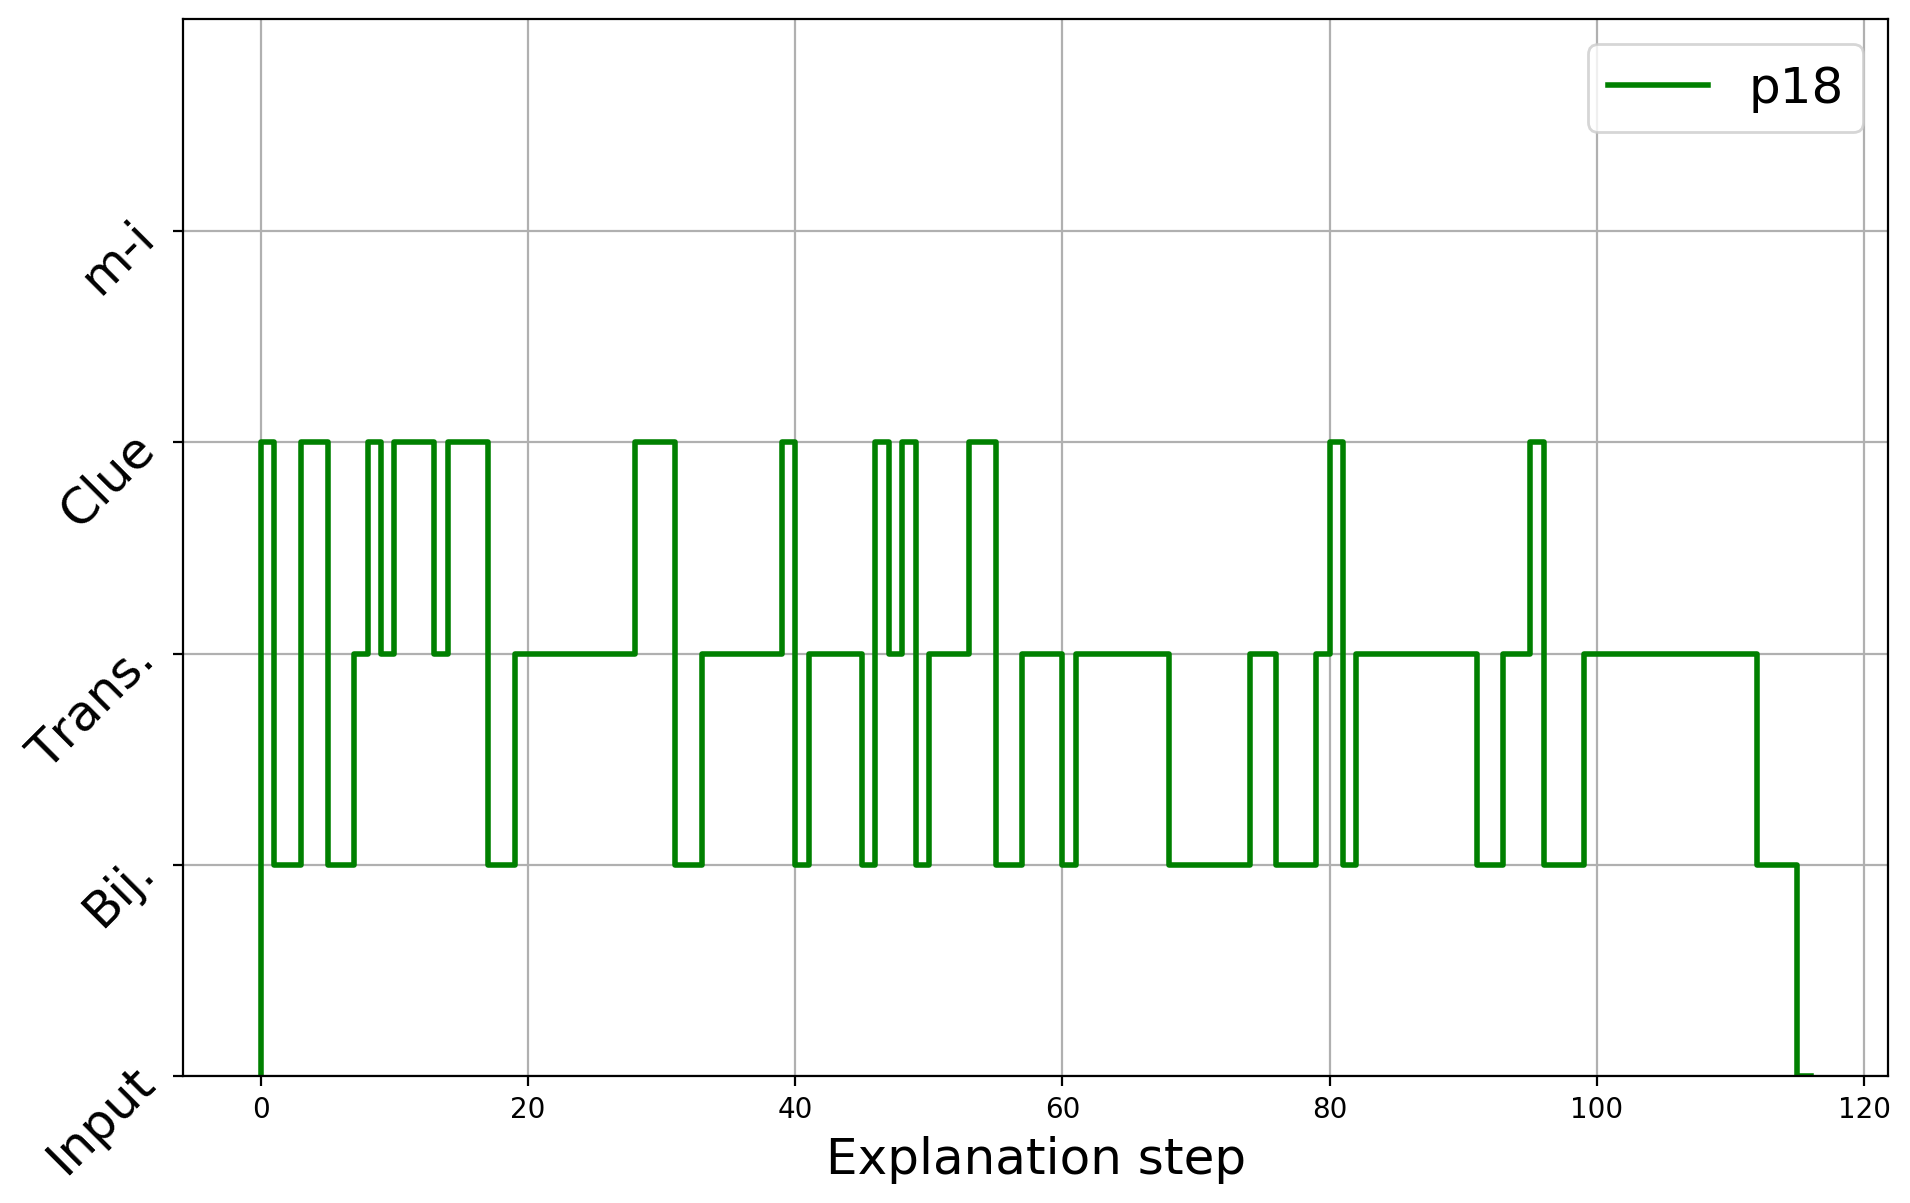
\includegraphics[width=0.32\linewidth]{figures/plot_cost_steps_p18}
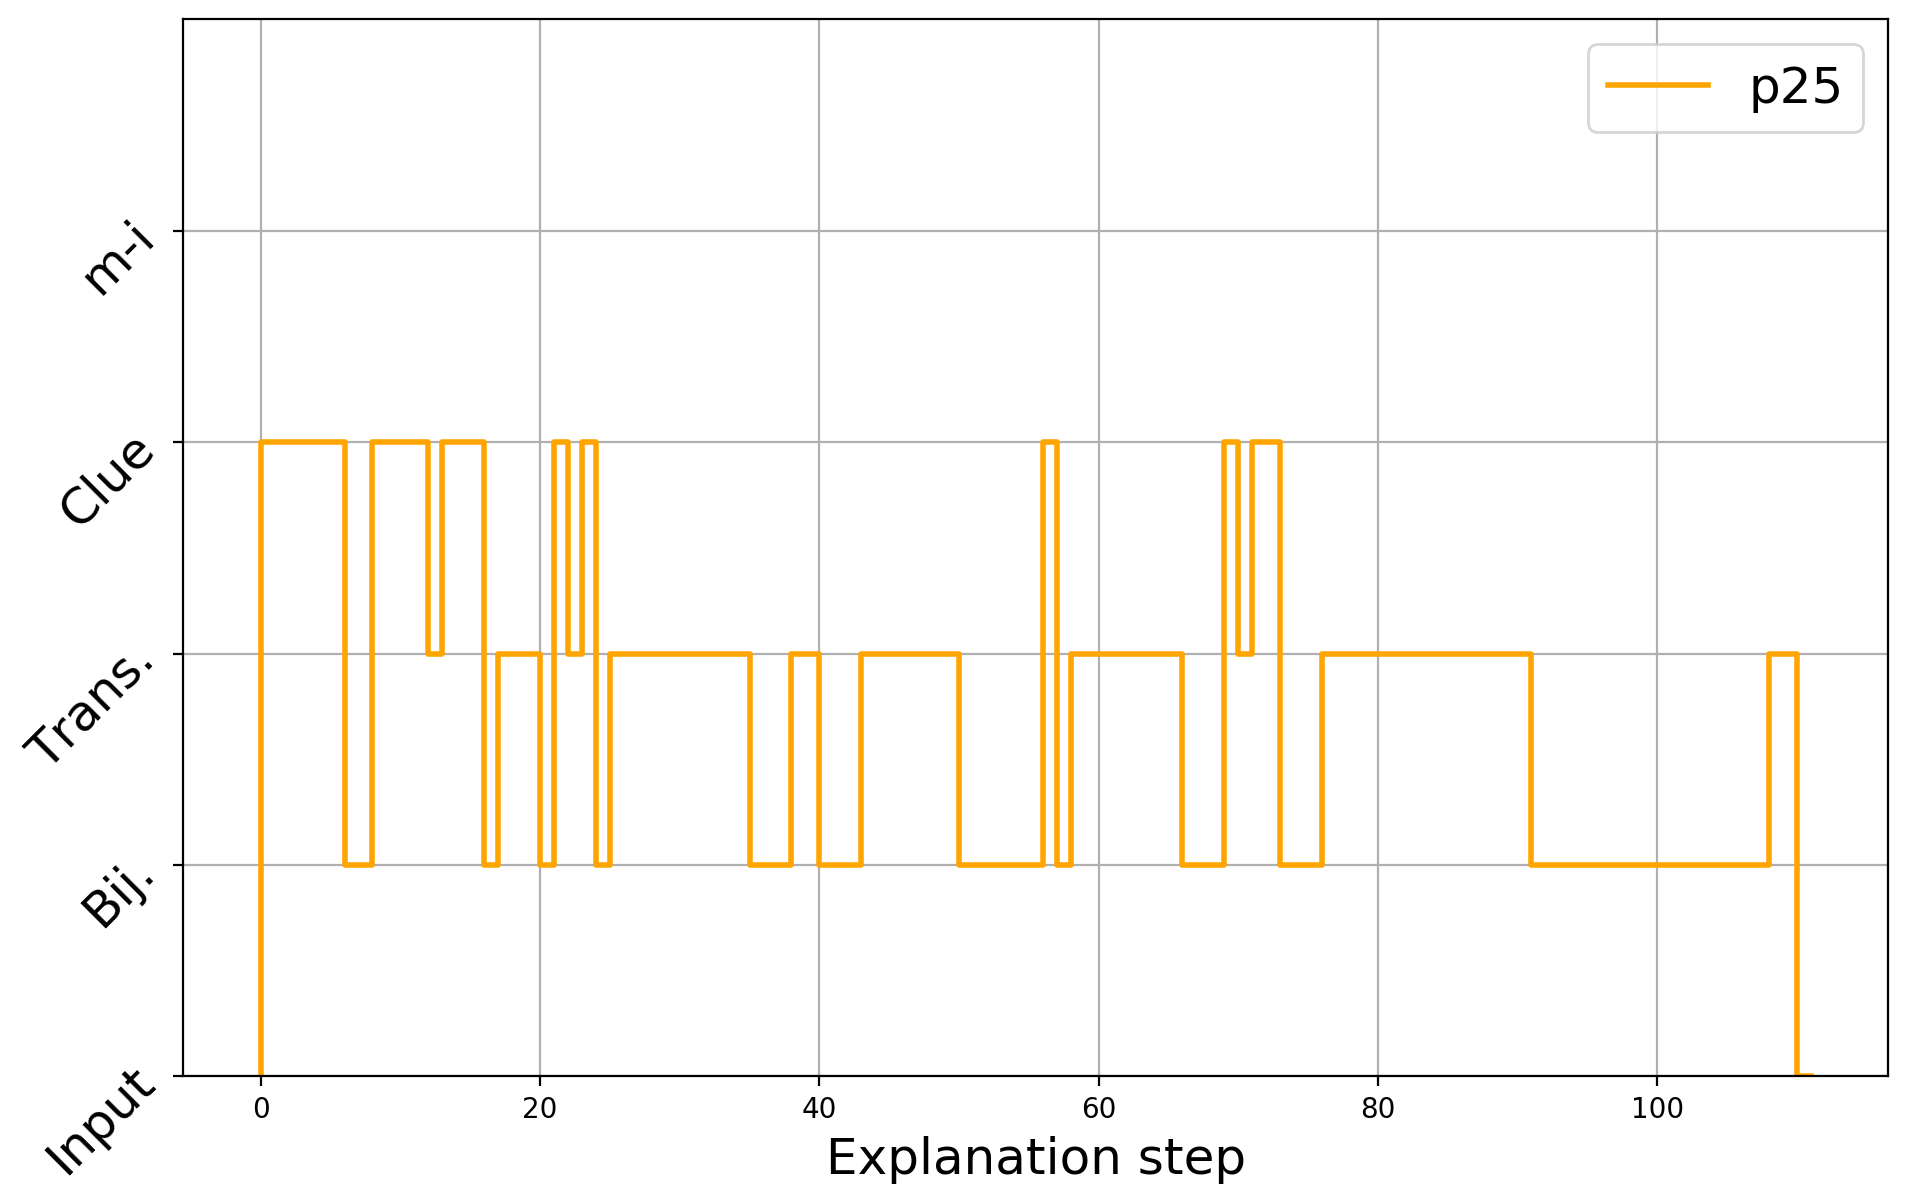
\includegraphics[width=0.32\linewidth]{figures/plot_cost_steps_p25}
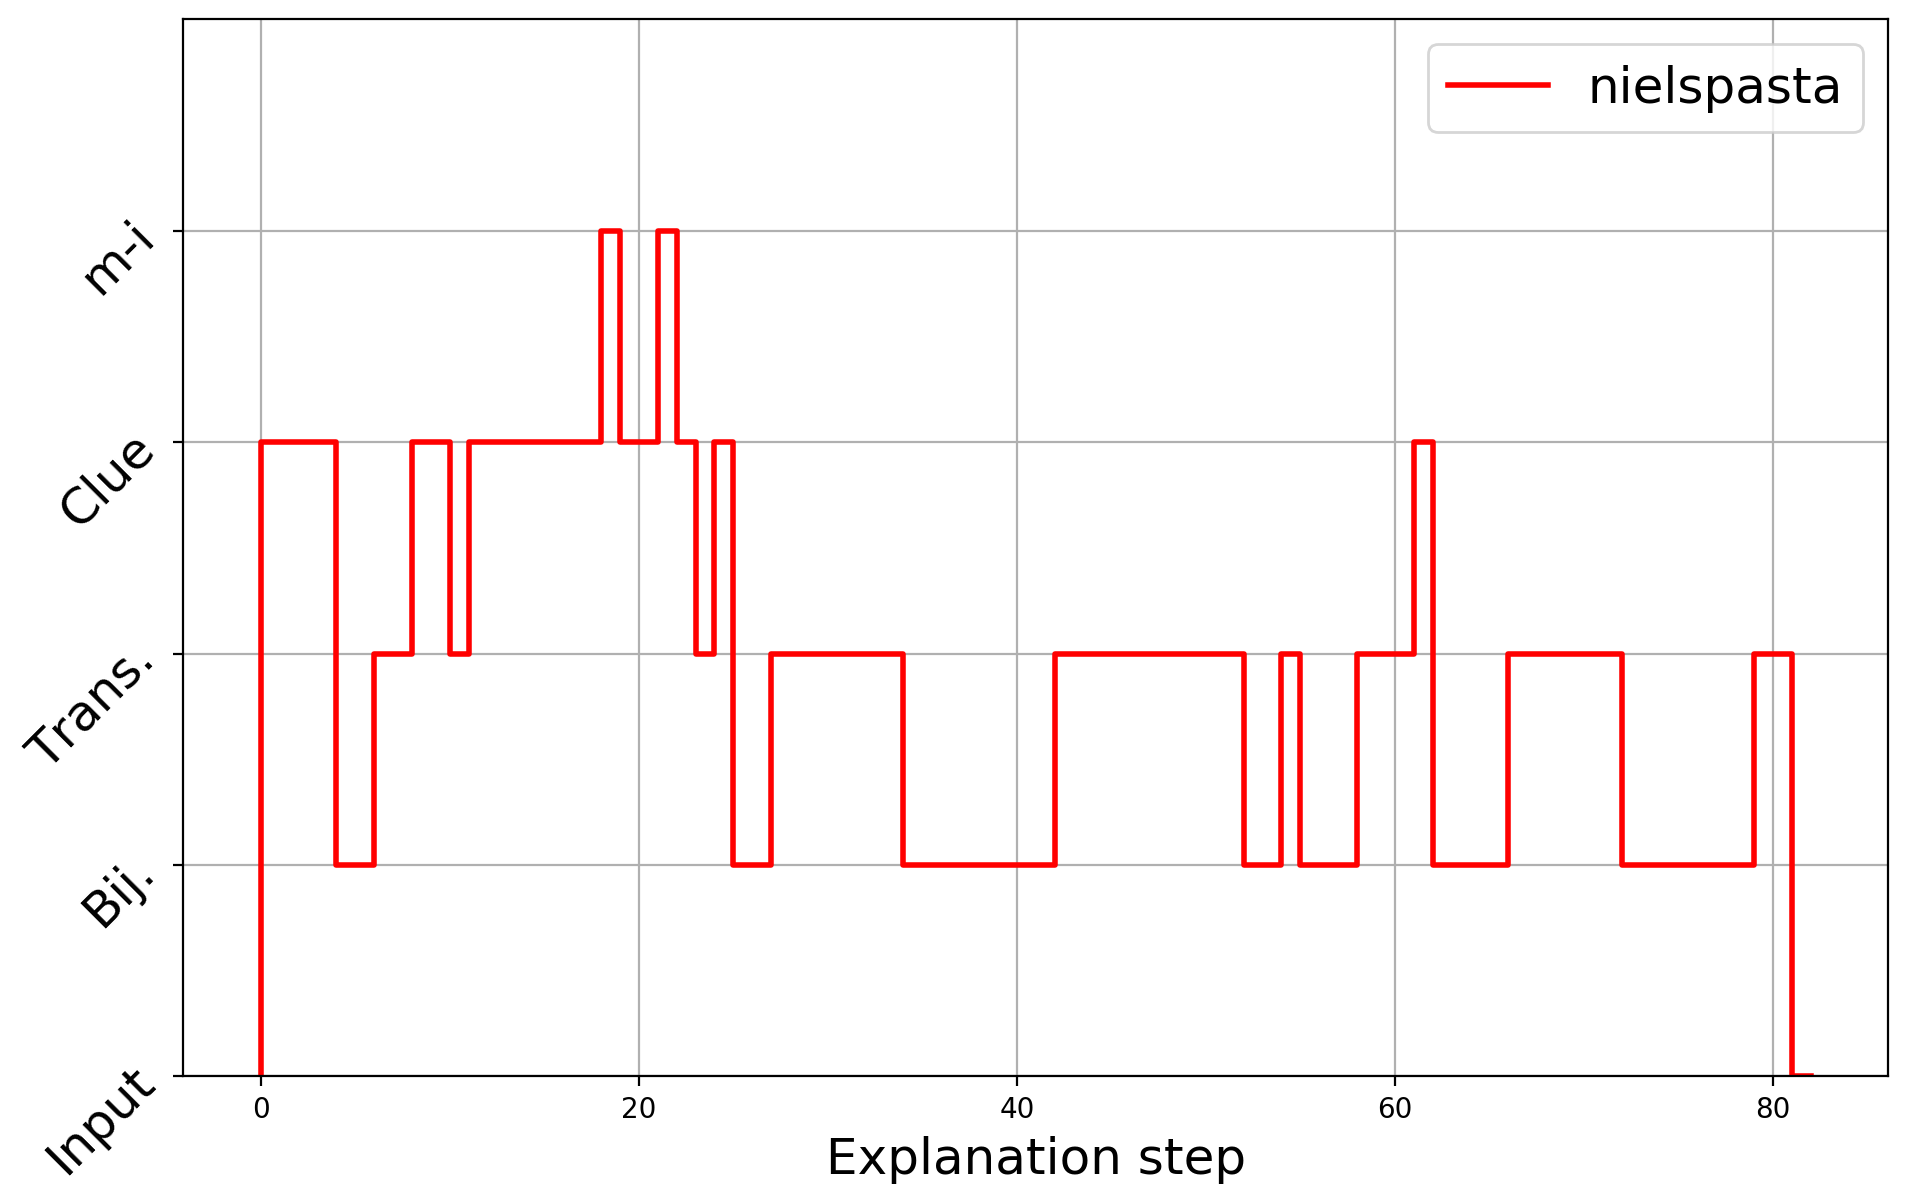
\includegraphics[width=0.32\linewidth]{figures/plot_cost_steps_nielspasta}\caption{Type of constraints used in each step}
\label{fig:steps}
\end{figure*}

\myparagraph{Sequence composition}
We first investigate the properties of the puzzles and the composition of the resulting sequence explanations. The results are shown in Table~\ref{table:composition}. The puzzle identified as p is our running example. $|type|$ is the number of types of entities (e.g. person, sauce) while $|dom|$ is the number of entities of each type. $|grid|$ is the number of cells in the grid, i.e.\ the number of literals in the maximal consequence interpretation $I_n=max(I_0,\allconstraints)$.
\begin{table}
	\centering
\begin{tabular}{c|ccc|c|cccccc} 
	\textbf{puzzle} & \textbf{$|$type$|$} & \textbf{$|$dom$|$} & \textbf{$|$grid$|$} & \textbf{steps} & \textbf{\% Bij.} & \textbf{\% Trans.} & \textbf{\% 1 Clue} & \textbf{\% m-i} & \textbf{\% m-c} \\ 
				\hline 
				%p5.output.json
				1 & 4 & 5 & 150 & 113 & 30.97 & 49.56 & 18.58 & 0.0 & 0\\ 
				%p16.output.json
				2 & 4 & 5 & 150 & 122 & 21.31 & 59.02 & 18.85 & 0.0 & 0\\ 
				%p12.output.json
				3 & 4 & 5 & 150 & 115 & 28.7 & 53.91 & 16.52 & 0.0 & 0\\ 
				%p18.output.json
				4 & 4 & 5 & 150 & 116 & 27.59 & 54.31 & 17.24 & 0.0 & 0\\ 
				%p19.output.json
				5 & 4 & 5 & 150 & 123 & 24.39 & 58.54 & 16.26 & 0.0 & 0\\ 
				%p20.output.json
				6 & 4 & 5 & 150 & 116 & 26.72 & 57.76 & 14.66 & 0.0 & 0\\ 
				%p25.output.json
				7 & 4 & 5 & 150 & 111 & 36.94 & 45.05 & 17.12 & 0.0 & 0\\ 
				%p93.output.json
				8 & 4 & 5 & 150 & 119 & 33.61 & 47.06 & 18.49 & 0.0 & 0\\ 
				%nielspasta.output.json
				p & 4 & 4 & 96 & 82 & 34.15 & 40.24 & 21.95 & 2.44 & 0\\ 
\end{tabular}  
\caption{Composition of puzzle explanations}
\label{table:composition}
\end{table}
Coincidentally, almost all the puzzles have 4 types with domain size 5,  
%  \todo{EMILIO: FIX, also the table!}, 
hence 150 cells, except for the pasta puzzle which has a domain size 4, thus 96 cells. We notice that the number of inference steps is around 120 for all but the pasta puzzle. When investigating the proportion of the inference steps that use bijections (only), transitivity (only) or a clue, we can see that around 50\% the explanations typically use a transitivity constraint, around 25\% typically a trivial bijectivity constraint (e.g. completing a row or column in one relation), and less then $1/5$th of the explanations actually need to use a clue.
In the table, \#m-i and \#m-c refer to the use of multiple implicit constraints and multiple clues respectively. We can see that it is never necessary to combine multiple constraints in one inference step. Also, notably, the puzzles from the booklet never require combining implicit constraints, while the anecdotally hard pasta puzzle is the only one that does: it cannot be solved by focussing on the clues but requires combining facts and knowledge in the table alone to crack it.

\myparagraph{Sequence progression} Figure \ref{fig:steps} shows a visualisation the type of explanation used at every step of the sequence, for some different puzzles. The red line is the pasta puzzle. We can see that typically at the beginning of the sequence, clues (4th line) and bijectivity (2nd line) are used, i.e., the trivial ones. This is then followed by a round of clues and some bijectivity/transitivity, after which a large fraction of the table can be completed with bijectivity/transitivty, followed by a few last clues and another round of completion.

The exception to this is the pasta puzzle. We can see that after around 20 steps where mostly clues have been used, twice a combination of implicit logigram constraints must be used to derive a new fact, after which the table can be easily completed with bijectivity/transitivity and twice the use of a clue.

\begin{table}
	\centering
	%\resizebox{\columnwidth}{!}{%
		\begin{tabular}{l|c|ccc|cccc} 
		    & \multicolumn{4}{c|}{\bf avg. facts} & \multicolumn{4}{c}{\bf \% of clue expl. with facts} \\
			\textbf{p} & \textbf{all} & \textbf{Clues} & \textbf{Trans.} & \textbf{Bij.} & \textbf{0 facts} & \textbf{1 fact} & \textbf{2 facts} & \textbf{$>$2 facts}\\ 
\hline
	%p5
	1 & 1.82 & 0.52 & 2.0 & 2.37 &66.6\% &28.5\% &0.0\% &4.7\% \\ 
	%p16
	2 & 1.80 & 0.61 & 2.0 & 2.38 &47.8\% &47.8\% &0.0\% &4.3\% \\ 
	%p12
	3 & 1.83 & 0.31 & 2.0 & 2.45 &78.9\% &15.7\% &0.0\% &5.2\% \\ 
	%p18
	4 & 1.85 & 0.45 & 2.0 & 2.50 &70.0\% &15.0\% &15.0\% &0.0\% \\ 
	%p19
	5 & 1.87 & 0.40 & 2.0 & 2.60 &65.0\% &30.0\% &5.0\% &0.0\% \\ 
	%p20
	6 & 1.82 & 0.29 & 2.0 & 2.35 &76.4\% &17.6\% &5.8\% &0.0\% \\ 
	%p25
	7 & 1.93 & 0.73 & 2.0 & 2.46 &57.8\% &26.3\% &5.2\% &10.5\% \\ 
	%p93
	8 & 1.84 & 0.18 & 2.0 & 2.57 &81.8\% &18.1\% &0.0\% &0.0\% \\ 
	%pasta
	p & 1.76 & 1.05 & 2.0 & 2.07 &60.0\% &15.0\% &0.0\% &25.0\% \\ 
		\end{tabular} 
	%}
	\caption{Puzzle explanation cost based on the cost function $f(I, C)$ and statistics on puzzle constraints}
	\label{table:sequence_leve}
\end{table}

\myparagraph{Explanation size}
Our cost-function is constructed to favour few (if any) clues and constraints in the explanations, and few previously derived facts $|E|$. Table~\ref{table:sequence_leve} shows the average number of facts used per explanation. We also show the average number of facts used when using only bijectivity or transitivity, or when a clue is used.

We can observe that the average number of facts used is indeed low, less than two. Furthermore, the breakdown shows that bijectivity typically uses more facts: it uses three `negative' facts in one row to infer a `positive' fact, as in Figure~\ref{fig:zebrascreen} or it uses one `positive' fact to infer three negative facts. Note that for such an intuitive constraint, the number of facts used does not matter much. Transitivity, by nature, always uses two previously derived facts. Finally, when looking at the number of facts used together with a clue we can see that our approach successfully finds small explanations: many clues (the trivial ones) use no facts, while some use 1 fact and only occasionally 2 or more facts are needed. The exception is again the difficult pasta puzzle.

\myparagraph{Nested sequence comparison}

\emilio{add intrepretaion of nested sequences experiments}
\begin{itemize}
	\item plot difference between step and nested sequence 
	\item length of the nested explanation sequence
	\item 
\end{itemize}

\begin{table}
	\centering
	\resizebox{\columnwidth}{!}{%
\begin{tabular}{lllllllll}
	\hline
	{} &     p & $\% steps w/ n-expl.$  & $\textbackslash \%$ steps use clues & $\textbackslash \#$ steps w/ 1 n-expl. & $\textbackslash \#$ steps w/ 2 n-expl. & $\textbackslash \#$ steps w/ $\>$2 n-expl. & avg. $max$(cost of expl in n-expl.) & avg. cost expl. w/ n-expl. \\
	\hline
	0 &  None &                       None &                 None &                         None &                         None &                          None &                                     None &                            None \\
	\hline
	\end{tabular}
	}
	\caption{Puzzle explanation cost based on the cost function $f(I, C)$ and statistics on puzzle constraints}
	\label{table:sequence_leve2}
\end{table}

\begin{figure*}[t]
	\centering
	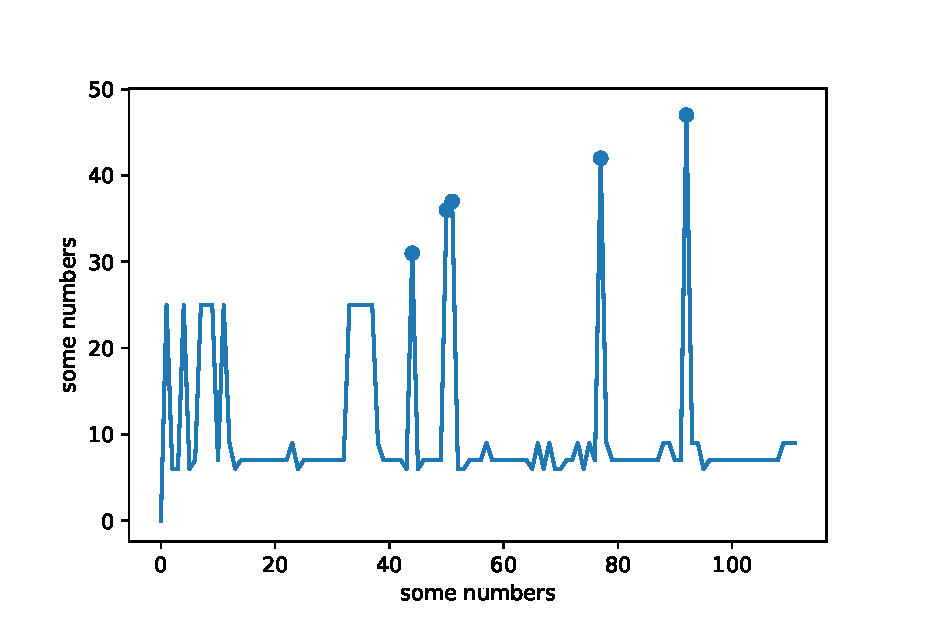
\includegraphics[width=0.5\linewidth]{figures/p18.eps}
	\caption{p18 cost with highlighted nested expl.}
	\label{fig:p18}
	\end{figure*}

	\begin{figure*}[t]
		\centering
		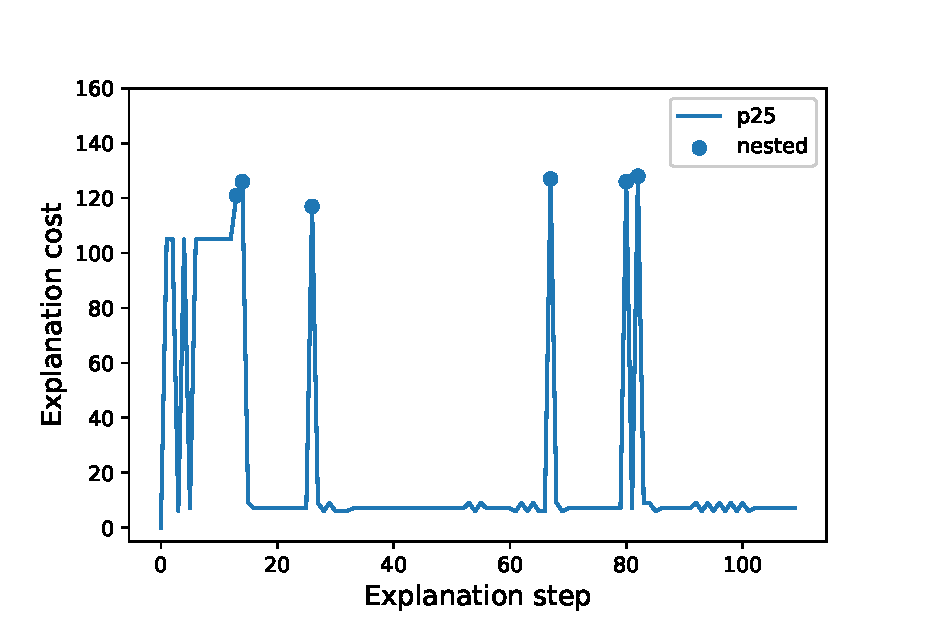
\includegraphics[width=0.5\linewidth]{figures/p25.eps}
		\caption{p25 cost with highlighted nested expl.}
		\label{fig:p25}
		\end{figure*}
		\begin{figure*}[t]
			\centering
			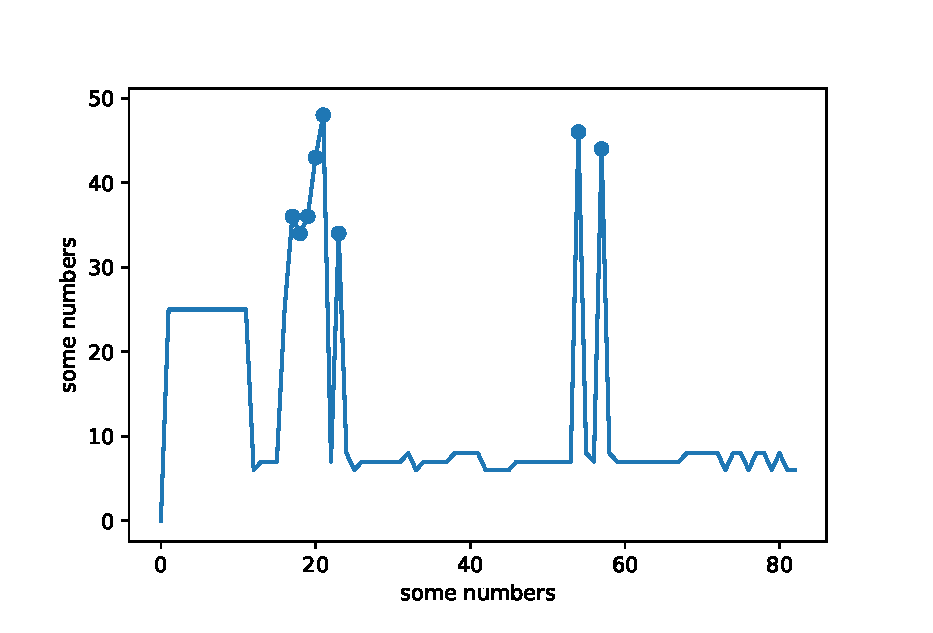
\includegraphics[width=0.5\linewidth]{figures/nielspasta-split-nested.eps}
			\caption{pasta cost with highlighted nested expl.}
			\label{fig:pasta}
			\end{figure*}